%%%%%%%%%%%%%%%%%%%%%%%%%%%%%%%%%%%%%%%%%%%%%%%%%%%%%%%%%%%%%%%%%%%%%
% LaTeX Template: Project Titlepage Modified (v 0.1) by rcx
%
% Original Source: http://www.howtotex.com
% Date: February 2014
% 
% This is a title page template which be used for articles & reports.
% 
% This is the modified version of the original Latex template from
% aforementioned website.
% 
%%%%%%%%%%%%%%%%%%%%%%%%%%%%%%%%%%%%%%%%%%%%%%%%%%%%%%%%%%%%%%%%%%%%%%

\documentclass[12pt]{report}
\usepackage[a4paper]{geometry}
\usepackage[myheadings]{fullpage}
\usepackage{fancyhdr}
\usepackage{lastpage}
\usepackage{graphicx, wrapfig, subcaption, setspace, booktabs}
\usepackage[T1]{fontenc}
\usepackage[font=small, labelfont=bf]{caption}
\usepackage{fourier}
\usepackage[protrusion=true, expansion=true]{microtype}
\usepackage[english]{babel}
\usepackage{sectsty}
\usepackage{url}
\usepackage{lmodern}
\usepackage[utf8]{inputenc}
\usepackage {tikz}
\usepackage{float}
\usetikzlibrary {positioning}
\usetikzlibrary{calc}

\definecolor{DarkGreen}{RGB}{0,140,0}
\definecolor{DarkBlue}{RGB}{0,0,160}
\definecolor{DarkRed}{RGB}{220,0,0}
\definecolor{DarkPurple}{RGB}{160,0,160}



\newcommand{\HRule}[1]{\rule{\linewidth}{#1}}
\onehalfspacing
\setcounter{tocdepth}{5}
\setcounter{secnumdepth}{5}

%-------------------------------------------------------------------------------
% HEADER & FOOTER
%-------------------------------------------------------------------------------
\pagestyle{fancy}
\fancyhf{}
\setlength\headheight{15pt}
\fancyhead[L]{Algorithmique Appliquée}
\fancyhead[R]{L. Giovannangeli, F. Jacques, J. Narboni}
\fancyfoot[R]{Page \thepage\ of \pageref{LastPage}}
%-------------------------------------------------------------------------------
% TITLE PAGE
%-------------------------------------------------------------------------------

\begin{document}

\title{ \normalsize \textsc{Algorithmique Appliquée}
		\\ [2.0cm]
		\HRule{0.5pt} \\
		\LARGE \textbf{\uppercase{Projet RoboCup}}
		\HRule{2pt} \\ [0.5cm]
		\normalsize \today \vspace*{5\baselineskip}}

\date{}

\author{
		Loann Giovannangeli, Fabien Jacques, Jonathan Narboni}

\maketitle
\renewcommand{\contentsname}{Sommaire}
\tableofcontents
\newpage

%-------------------------------------------------------------------------------
% Section title formatting
\sectionfont{\scshape}
%-------------------------------------------------------------------------------

%-------------------------------------------------------------------------------
% BODY
%-------------------------------------------------------------------------------

\part*{Modélisation du Problème}

L'objectif de ce projet est de trouver une modélisation du problème de défense d'un but lors de la RoboCup. Ce problème consiste à trouver une manière optimale de placer les défenseurs par rapports à l'emplacement de leur but et des attaquants.

Ce document présente les premières idées de modélisation que nous avons après les premiers TD.\\

Voici comment nous modélisons le problème :
\newline
\newline
\chapter{Entrées}
Les entrées de notre problème sont les informations qui nous intéressent sur nos robots et le terrain. Elles nous permettront de simuler la réalité dans nos algorithmes afin que nos résultats aient un sens concret.\\

Soient :
\begin{itemize}
\item $o_i \in O$ ($i \in \{1,..., n\}$) Les $n$ adversaires. On notera $o_i.x$ et $o_i.y$ les coordonnées de $o_i$.
\item $d_i \in D$ ($i \in \{1,..., k\}$) Les $m$ défenseurs.
\item $\theta_{step}$ Pas de discrétisation pour les angles de tirs. On considérera "l'angle $k$" comme étant un angle de mesure $k \times \theta_{step}$ radians. On nommera $K_{max}$ le k maximum tel que $k \times \theta_{step} $<$ 2 \pi$.
\item $pos_{step}$, $X_{max}$, $Y_{max}$, Pas de discrétisation pour les positions sur le terrain, Abscisse  maximale et Ordonnée maximale. On considérera qu'un robot est en position $(x, y) \in (N \times N)$ si il est en position ($x \times pos_{step}$, $y \times pos_{step}$).
\end{itemize}

\chapter{Fonctions nécessaires}
\begin{itemize}
\item $cadre(x, y, k)$ ($x, y, k \in N$) Fonction qui renvoie vrai si le tir d'un attaquant aux coordonnées $(x, y)$ d'angle $k$ est bien cadré et faux sinon.
\item $interception(x, y, k, x', y')$ Fonction qui renvoie vrai si le tir d'un attaquant en (x, y) d'angle k est arrêté par un défenseur en (x', y') et faux sinon.
\end{itemize}
\space
\space

\chapter{Graphe} \bigbreak
On crée le graphe G suivant :\\
\begin{figure}[H]
	\centering
	\scalebox{1.3}
	{
		
		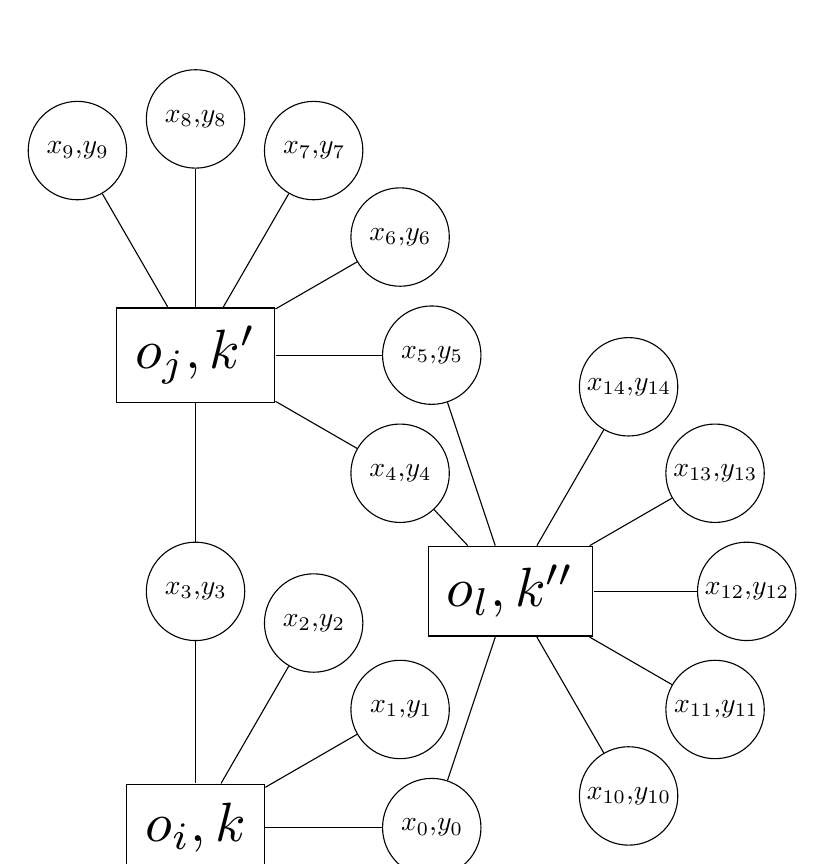
\begin{tikzpicture}[scale=2, transform shape,atq node/.style={shape=rectangle,scale=1,draw=black},def node/.style={scale=0.5, shape=circle,draw=black,inner sep=0,text width=35,align=center}, ]
		\node[atq node] (atq1) at (0,0){$o_i,k$};
		\node[atq node] (atq2) at (0,3){$o_j,k'$};
		\node[atq node] (atq3) at (2,1.5){$o_l,k''$};
		\newcounter{nDef};
		%def position + basic path
		\foreach \x in {0,...,3}
		{
			\node[def node] (d\arabic{nDef}) at ($(atq1)+(\x*30:1.5)$){$x_{\arabic{nDef}}$,$y_{\arabic{nDef}}$};
			\path (atq1) edge (d\arabic{nDef});
			\stepcounter{nDef};
			
		}
		\foreach \x in {11,...,16}
		{
			\node[def node] (d\arabic{nDef}) at ($(atq2)+(\x*30:1.5)$){$x_{\arabic{nDef}}$,$y_{\arabic{nDef}}$};
			\path (atq2) edge (d\arabic{nDef});
			\stepcounter{nDef};
			
		}
		\foreach \x in {10,...,14}
		{
			\node[def node] (d\arabic{nDef}) at ($(atq3)+(\x*30:1.5)$){$x_{\arabic{nDef}}$,$y_{\arabic{nDef}}$};
			\path (atq3) edge (d\arabic{nDef});
			\stepcounter{nDef};
			
		}
		
		%additionnal path
		\path (atq2) edge (d3);
		\path (atq2) edge (d3);
		\path (atq3) edge (d0);
		\path (atq3) edge (d4);
		\path (atq3) edge (d5);
		
		
		
		
		
		\end{tikzpicture}
		
	}
\caption{Exemple de modélisation avec 3 tirs possibles: ici \{($x_3,y_3$), ($x_5,y_5$)\} est une solution.}
\end{figure}
\section{Sommets attaquants}
$\forall i \in \{1, ..., n\}$, $\forall k \in \{0, ..., K_{max} \}$

Si $cadre(o_i.x, o_i.y, k)$ est vrai : on ajoute un sommet au graphe d'étiquette (i, k) qui représente un tir possible de l'attaquant $o_i$. \bigbreak

\section{Sommets défenseurs}
$\forall x \in \{1, ..., X_{max}\}$ $\forall y \in \{1, ..., Y_{max}\}$ 

Pour tout sommet d'étiquette (i, k) tel que $intercepte(o_i.x, o_i.y, k, x, y)$ : On crée un sommet d'étiquette (x, y) qui représente un défenseur placé en (x, y) si ce sommet n'existe pas déjà et on ajoute une arête entre $(i, k)$ et $(x, y)$ qui représente le fait qu'un défenseur placé en $(x, y)$ arrêterai le tir $(i, k)$.

\chapter{Solution du problème}
Une solution du problème est un ensemble de taille minimal de sommets défenseurs qui domine l'ensemble des sommets attaquants.
Pour trouver cet ensemble on peut essayer avec 1, puis 2, puis 3, etc. On sait qu'on pourra toujours trouver un ensemble de taille n (nombre d'attaquants) car un défenseur est capable de bloquer tous les tirs d'un attaquant en se plaçant suffisamment proche de lui. 

\chapter{Extensions}
\section{Gestion des collisions}
Si on veut éviter d'avoir des robots qui rentrent en collision, on peut ajouter une arête entre chaque paire de sommets défenseurs pour lesquels avoir un défenseur sur chacune des positions causerai une collision. Une solution du problème qui évite les collisions doit alors avoir comme condition supplémentaire d'être un ensemble de sommets stable.\\
Le graphe du problème devient alors:\\ \bigbreak
\begin{figure}[H]
	\centering
	\scalebox{1.3}
	{
		
		\begin{tikzpicture}[scale=2, transform shape,atq node/.style={shape=rectangle,scale=1,draw=black},def node/.style={scale=0.5, shape=circle,draw=black,inner sep=0,text width=35,align=center},coll edge/.append style={color=DarkRed,line width=1.5}]
		\node[atq node] (atq1) at (0,0){$o_i,k$};
		\node[atq node] (atq2) at (0,3){$o_j,k'$};
		\node[atq node] (atq3) at (2,1.5){$o_l,k''$};
		\setcounter{nDef}{0}
		%def position + basic path
		\foreach \x in {0,...,3}
		{
			\node[def node] (d\arabic{nDef}) at ($(atq1)+(\x*30:1.5)$){$x_{\arabic{nDef}}$,$y_{\arabic{nDef}}$};
			\path (atq1) edge (d\arabic{nDef});
			\stepcounter{nDef};
			
		}
		\foreach \x in {11,...,16}
		{
			\node[def node] (d\arabic{nDef}) at ($(atq2)+(\x*30:1.5)$){$x_{\arabic{nDef}}$,$y_{\arabic{nDef}}$};
			\path (atq2) edge (d\arabic{nDef});
			\stepcounter{nDef};
			
		}
		\foreach \x in {10,...,14}
		{
			\node[def node] (d\arabic{nDef}) at ($(atq3)+(\x*30:1.5)$){$x_{\arabic{nDef}}$,$y_{\arabic{nDef}}$};
			\path (atq3) edge (d\arabic{nDef});
			\stepcounter{nDef};
			
		}
		
		%additionnal path
		\path (atq2) edge (d3);
		\path (atq2) edge (d3);
		\path (atq3) edge (d0);
		\path (atq3) edge (d4);
		\path (atq3) edge (d5);
		
		%collision path
		\path (d4) edge[coll edge] (d5);
		\path (d3) edge[coll edge] (d5);
		\path (d3) edge[coll edge] (d2);
		\path (d2) edge[coll edge] (d1);
		\path (d3) edge[coll edge,bend right] (d1);
		\path (d6) edge[coll edge, bend left] (d14);
		
		
		\end{tikzpicture}
		
	}
	\caption{Modélisation des collision: les arêtes représentant les collisions sont en rouge, ici, \{($x_3,y_3$), ($x_5,y_5$)\} n'est plus solution, car ils sont adjacents; par contre \{($x_3,y_3$), ($x_0,y_0$)\} est une solution.}
\end{figure}


%-------------------------------------------------------------------------------
% REFERENCES
%-------------------------------------------------------------------------------
%\newpage
%\section*{References}
%\addcontentsline{toc}{section}{References}

\end{document}